\documentclass[
    % notes,
    aspectratio=169
]{beamer}
\hypersetup{unicode=true} % fix "PD1 encoding, removing `\CYRI'"
\usepackage[utf8]{inputenc}
\usepackage[T2A,T1]{fontenc}
\usepackage[english,russian]{babel}

\usepackage{caption}
\usepackage{subcaption}

\graphicspath{{../figures}}

\newcommand{\tr}[1]{\mathrm{Tr} \left\{ #1 \right\}}
\newcommand{\sx}{I_\mathrm{x}}
\newcommand{\sy}{I_\mathrm{y}}
\newcommand{\sz}{I_\mathrm{z}}
\newcommand{\hdz}{H_\mathrm{dz}}


\setbeamertemplate{caption}[numbered] % number figures

\usetheme{Madrid}

\title[Многочастичная запутанность]{Многочастичная запутанность}
\subtitle{в многоквантовой спектроскопии ЯМР в твердом теле}
\author[Лазарев И.Д.]{\textbf{И.Д. Лазарев\inst{1,2}}}

\institute[МГУ, ИПХФ РАН]
{
  \inst{1}%
  Московский государственный университет им. М. В. Ломоносова
  \and
  \inst{2}%
  Институт проблем химической физики РАН
}

\date[2022]{Июнь 2022}


\begin{document}

\frame{\titlepage}
\note{
    Еще раз добрый день, коллеги!
    Я веду свою научную работу в Черноголовке
    в ИПХФ РАН в теоретическом отделе
    в лаборатории спиновой динамики и спинового компютинга
    под руководством Фельдмана Эдуарда Беньяминовича

    Тема моей работы: Многочастичная запутанность...

    Почему это важно?
    Квантовые корреляции ответственны за преимущества квантовых приборов и устройств над их классическими аналогами.
    Такие корреляции отсутствуют в классической физике.
    Изучение их свойств и методов управления ими является теоретической основой квантовых технологий.

    Почему ЯМР?
    Потому что в твердотельном ЯМР можно значительно продвинуться в этом направлении.
}

% \AtBeginSection[] {} % show display table of contest before new section
\begin{frame}
\frametitle{План доклада}
\tableofcontents
\end{frame}
\note{
  План доклада будет стандартным.
  В начале будет обсуждена проблематика и ее предпосылки,
  а также будет поставлена цель исследования.
  Следом будет представлен методы и работы на которые оприрается данная работа.
  Затем я сделаю краткий обзор основных полученных результатов.
}

\section{Введение}
\chapter*{Введение}
\addcontentsline{toc}{chapter}{Введение}

% Во введении к диссертации определяется актуальность избранной темы, степень ее разработанности, цели и задачи, объект и предмет исследования, научная новизна, теоретическая и практическая значимость работы, методология диссертационного исследования, положения, выносимые на защиту, степень достоверности и апробация результатов.

% актуальность темы исследования
%   - Квантовые технологии.
%   - Квантовое превосходство.
%   - Квантовая теория информации.
%   - Запутанность в фундаментальных исследованиях.
%   - Квантовые симуляторы и квантовые компьютеры
%
% - степень ее разработанности
%   - История бинарной запутанности
%   - Критерии бинарной запутанности
%   - Эксперименты с бинарной запутанностью
%   - ?? Работы по многочастичной запутанности
%
% - цели и задачи
%   - Разработать теорию МК динамики для системы эквивалентных спинов.
%   - Исследовать многочастичную запутанность в системе эквивалентых спинов.
%   - Исследовать многочастичную запутанность в системе эквивалентных спинов с дипольно упорядоченным начальным состоянием.
%   - Исследовать многочастичную запутанность в одномерной системе.
%   - Разработать экспериментальный метод для определения информации Вигнера-Янасе в МК экcперименте ЯМР.
%   - Провести сравнение результатов оценки многочастичной запутанности на основе информации Вигнера-Янасе и информации Фишера.
%
% - научная новизна
%   - Оценка количества запутанных спинов
%   - Определение информации Вигнера-Янасе
%
% - теоретическую и практическую значимость работы;
%
% - методологию и методы исследования; ??
%
% - положения, выносимые на защиту;
%
% - степень достоверности и апробацию результатов. ??
%
%
% Nowadays, it has been recognized that most physical
% processes in nature can be formulated in terms of processing of information, and information may be central
% to understanding quantum theory [19].
%
%
% проблема классификации и количественной оценки запутанности в целом на сегодняшний день все еще далека от полного понимания.

% Such an investigation of many-spin entanglement is performed for the first time.


\section{Исследование квантовых корреляции методами ЯМР}

\subsection{Многочастичная запутанность}
\begin{frame}{Многочастичная запутанность}
  $$
  \left| \Psi_{3-\mathrm{ent}} \right\rangle
  = \frac{1}{\sqrt{8}}
  \left| \uparrow_1 \right\rangle
  \otimes
  \left(
    \left| \uparrow_2\uparrow_4\right\rangle +
    \left|\downarrow_2\downarrow_4\right\rangle
  \right)
  \otimes
  \left(
    \left|\uparrow_3\uparrow_5\uparrow_9\right\rangle +
    \left|\downarrow_3\downarrow_5\downarrow_9\right\rangle
  \right)
  \otimes
  \left(
    \left|\uparrow_6\uparrow_7\uparrow_8\right\rangle +
    \left|\downarrow_6\downarrow_7\downarrow_8\right\rangle
  \right)
  $$
  \begin{alertblock}{Многочастичная запутанность $k$-частиц}
  $$
  \left| \Psi_{k-\mathrm{ent}} \right\rangle
  	= \otimes^\mathrm{M}_{i=1} \left| \Psi_{i} \right\rangle,
  $$
  где $\left| \Psi_{i} \right\rangle$ это состояние подсистемы с $N_i$ частицами,
  $ \sum\limits_{i=1}^N N_i = N $
  и $ \exists m: N_{m} \ge k$
  \end{alertblock}

\end{frame}
\note{
  А вот многочастичная запутанность изучена гораздо хуже,
  так как для этого нужно исследовать многочастичные системы,
  пространство которой экспоненциально растет с увеличение числа частиц.

  Также не очевидно какое определение должнобыть у многочастичной запутанности.

  В нашей работе мы используем для многочастичной запутанности  следующее определение: ...слайд...

  То есть наличие запутанности порядка $k$,
  говорит о том что существует несепарабельная подсистема размера $k$.
}

\begin{frame}{Меры многочастичной запутанности}
  \vspace{-2mm}
  \begin{block}{Свойства}
    \begin{enumerate}
      \item $
        F(\rho_1 \otimes \rho_2 ,H_1 \otimes I_2 + I_1 \otimes H_2)
    	= F_{1} (\rho_1, H_1) + F_{2} (\rho_2 , H_2)
      $
      \item $F \leq N^2$
    \end{enumerate}
  \end{block}
  \vspace{-1mm}
  \begin{alertblock}{Уточнение верхней границы величины $F$}
    Пусть в системе максимальный размер несепарабельной подсистемы равен $k$, тогда
    $$ F^{k} \leq \left[ \frac N k \right] k^2 + \left(N - k \left[ \frac N k \right]\right)^2 $$
  \end{alertblock}
  \vspace{-1mm}
  \begin{examples}
    \begin{enumerate}
      \item Косая информация Вигнера-Янасе\footnote[frame]{Zeqian Chen \textit{Phys. Rev. A} \textbf{71}, 052302 (2005)}
      \item Квантовая информация Фишера\footnote[frame]{P. Hyllus et al. \textit{Phys. Rev. A} \textbf{85}, 022321 (2012)}
    \end{enumerate}
  \end{examples}
\end{frame}
\note{
 В настоящее время признано, что большинство физических процессов в природе можно сформулировать в терминах обработки информации, и концепция информации может быть центральной для понимания квантовой теории.


Нас интересует два свойства меры:
1. В сепарабельной системе с матрицей плотности $\rho = \rho_1 \otimes \rho_2$ квантовая информация Фишера удовлетворяет условию аддитивности)
2. Известна ее верхняя граница $F_\mathrm{Q} \leq N^2$, где $N$ это количество частиц в системе.

Благодаря этим свойствам, зная величину меры в системе можем оценить нижнюю границу количества запутанных частиц в системе. То есть если в системе максимальный размер не сепарабельной подистемы равен $k$, то
мера такой всей системы точно не больше данного значеничя: ...слайд...

Таким образом получив значение меры  выше при фиксированом $k$ ...слайд...,  мы можем утверждать что существует несепарабельная системы размера больше $k$ расчитать дать нижнюю оценку на минимальный размер несепарпбельной системы.

Какие величины имееют такие свойства?
В квантовой теории информации есть ...слайд...
Эти величины сами по себе очень интересные.
}


% \begin{frame}{Меры многочастичной запутанности}
% Фиксируем какое-то значение $k$ - максимальное количество спинов в несепарабельной подсистеме
% $$ N > k \geq N_1 \geq N_2 \geq \dots \geq N_l, \quad \sum_{i=0}^{l} N_i = N, $$
% где $l$ количество несепарабельных подсистем.
%
% Верхняя граница информации Фишера для такой системы:
% $$
% F^k = F_{1} + \dots + F_{l}
% \leq N^2_1 + \dots + N^2_e
% \leq \underbrace{
% 	k^2 + k^2 + \dots + k^2
% 	}_{m = \left[\frac N k \right] \, \mbox{раз}}
% 	+ \underbrace{(N-km)^2}_{\mbox{остаток}}
% $$
%
% \begin{alertblock}{}
%     $$  F^k \leq \left[ \frac N k \right] k^2 + \left(N - k \left[ \frac N k \right]\right)^2 $$
% \end{alertblock}
% \end{frame}
% \note{
% Доказательства этого факта сводится к вычислению верхней границы квантовой информации Фишера для с фиксированым размером не сепарабельных подсистем.
% Мы для себя фиксируем какое-то значение $k$ - максимальное количество спинов в несепарабельной подсистеме. Сделаем оценку сверху для информации Фишера.
%
% Пусть есть я ...
%
% Рассмотрим пару подсистем для которых верно $k > N_i > N_{i-1} > 0$.
% Квантовая информации Фишера этих двух подсистем:
% $$
% F_{Q\,i,i-1} \leq N_{i}^2 + N_{i-1}^2
% $$
% При этом если мы рассмотрим случай когда в правой системе на один спин меньше, а в левой на одим больше то оценка верхней границы будет выше:
% $$
% \bar F_{Q\,i,i-1}
% 	\leq \left( N_{i}^2 + 1 \right)
% 		+ \left( N_{i-1}^2 - 1\right)
% 	\leq N_{i}^2 + N_{i-1}^2
% 		+ 2 \left(N_{i} - N_{i-1} + 1 \right)
% $$
% Следовательно в худшем случае...???
%
% Следовательно если мы подсчитаем информацию Фишера, то мы
% можем дать нижнюю границу количества запутанных частиц.
% }

\subsection{Квантовая информация Фишера}
\begin{frame}{Квантовая информация Фишера}
  \begin{block}{}
    Квантовая информация Фишера\footnote[frame]{D. Petz and C. I Ghinea, \textit{Quantum Probab. Relat. Top.} (2011)}
    показывает,
    как быстро изменяется квантовое состояние,
    определяемое матрицей плотности,
    при изменении некоторого параметра.
  \end{block}
  Квантовая информация Фишера --- это прямой аналог классической информации Фишера и основная мера в квантовой метрологии.
  Квантовая информация Фишера $F_Q$ для матрицы плотности $\rho$ по отношению к наблюдаемой $A$:
  $$
    F_Q \left(\rho, A \right) =
      2\sum_{j,k} \frac{\left(\lambda_j - \lambda_k \right)^2}
        {\lambda_j + \lambda_k}
      \left| \langle j|A|k \rangle \right|^2,
  $$
  где $\lambda_k$ и $|k \rangle$ --- собственное значение и собственный вектор матрицы плотности $\rho$.
\end{frame}
\note{
    Квантовая информация Фишера показывает, 
    как быстро изменяется квантовое состояние, 
    определяемое матрицей плотности, 
    при изменении некоторого параметра. 
    Как правило этот параметр является временем эволюции квантового состояния.

    Квантовая информация Фишера --- это прямой аналог классической информации Фишера, 
    и так как это скорость изменения состояния при изменении параметра часто используется в квантовой метрологии. 

    Далее мы сосредоточимся на квантовой информации Фишера. 
    так как для нее в МК эксперименте ЯМР возможно получить оценку снизу.
}


\subsection{Косая информация Вигнера-Янасе}
\section{Косая информация Вигнера-Янасе}
\label{sec:skew-wigner-yanase-information}
% история
% определение
% применение
% свойства
% формула
% связь c информацией Фишера
% связь со вторым моментом

% 10.1103/PhysRevLett.91.180403 Inro
% В исследовании измерения квантовомеханических операторов Вигнер показал, что наблюдаемые, которые не коммутируют с аддитивной сохраняющейся величиной, труднее измерить, чем те, которые коммутируют с сохраняющейся величиной; то есть, наличие закона сохранения накладывает ограничение на измерение наблюдаемых, которые несовместимы (не коммутируют) с сохраняющейся величиной [1,2]. Араки и Янасе строго установили, что наблюдаемые величины, не совпадающие с сохраняющейся величиной, не могут быть измерены точно (в смысле фон Неймана), возможно только приближенное измерение, и существует компромисс между "размером" измерительного прибора и точностью измерения [3,4]. Это составляет знаменитую теорему Вигнера-Араки-Янасе, которая накладывает принципиальное ограничение на измерение квантовомеханических наблюдаемых. Эта теорема в дальнейшем исследовалась многими авторами [5-9].
% Cледовательно наблюдаемые величины,
% которые коммутируют с аддитивными сохраняющимися величинами
% (энергия, компоненты линейного и углового моментов, электрический заряд),
% могут быть измерены с помощью микроскопических аппаратов,
% а те, которые не коммутируют с этими величинами, требуют для своего измерения макроскопических систем\cite{Wigner1960}.

%
%Согласно квантовомеханической теории,
% екоторые наблюдаемые величины могут быть измерены гораздо легче, чем другие:

Араки и Янасе строго установили, что наблюдаемые величины,
которые не являются интегралами движения,
не могут быть измерены точно (в смысле фон Неймана),
и возможно только приближенное измерение.
Согласно знаменитой теореме Вигнера-Араки-Янасе, которая накладывает принципиальное ограничение на измерение квантовомеханических наблюдаемых,
существует компромисс между ``размером'' измерительного прибора и точностью измерения\cite{Araki1961, Ozawa1991, Ozawa2002a, Ozawa2002b, Matsumoto1993, Kakazu3469}.
Наблюдаемые величины,
которые коммутируют с аддитивными сохраняющимися величинами
(энергия, компоненты линейного и углового моментов, электрический заряд),
могут быть измерены с помощью микроскопических аппаратов;
те же, которые не коммутируют с этими величинами, требуют для своего измерения макроскопических систем\cite{Wigner1960}.
Отсюда возникает проблема определения меры наших знаний относительно последних.

% Theoretical and Mathematical Physics, 202(1): 104–111 (2020)
Косая информация\cite{Wigner1963} была введена Вигнером и Янасе
в контексте квантовых измерений в качестве меры информации,
содержащейся в векторе квантового состояния, лежащего под углом по отношению к наблюдаемой $A$.
\begin{equation}\label{eq:wyi}
  I_{WY}(\rho, A)
  = -\frac{1}{2} Tr([\sqrt{\rho}, A])^2
  = Tr(\rho A^2) - Tr(\sqrt \rho A \sqrt \rho  A ).
\end{equation}
%
В частности, если $\rho = \ket{\psi}\bra{\psi}$ чистое состояние, тогда
%
\begin{equation}
  I_{WY}(| \psi \rangle, A)
  = \langle \psi | A^2 | \psi \rangle - \langle \psi | A| \psi \rangle ^2
\end{equation}

Косая информация Вигнера-Янасе существенно отличается от энтропии фон Неймана \cite{Wigner1960, Lieb1973prl, Lieb1973, Wehrl1978},
но глубоко связана с ней.
Энтропия, как ее обычно определяют, является мерой нашего незнания\cite{Weaver1949}.
Это мера, в которой знания о любой наблюдаемой величине находятся в одном ряду.
С точки зрения энтропии информационное содержание всех чистых состояний,
которые могут быть описаны одним вектором состояния, одинаково.
Это неверно для косой информации Вигнера-Янасе.
В отличие от вектора консервативной величины наблюдаемой $A$,
вектор состояния, лежащего наклонно к наблюдаемой $A$, содержит информацию.

Позднее было признано, что косая информация,
помимо своего изначального значения как меры информационного содержания состояний,
допускает также несколько интерпретаций,
носящих более физический и теоретико-информационный характер.
Например, Шунь Лун Ло показал\cite{Luo2003, Luo2005, Luo2005pra, Luo2006, Luo2017} ,
что косую информацию Вигнера-Янасе можно интерпретировать
как квантовую неопределенность наблюдаемой $A$ для квантового состояния $\rho$.

Интригующей и тонкой особенностью косой информации является использование в ней квадратного корня из оператора плотности квантового состояния.
Тем не менее популярность получили и естественные модификации косой информации Вигнера-Янасе,
в которых нет корня из оператора плотности.
Например, величина
%
\begin{equation}\label{eq:wyi-modification-l}
  L(\rho, A)
  = -\frac{1}{2} Tr([\rho, A])^2.
\end{equation}
%
Значительным преимуществом величины $L(\rho, A)$ в сравнении с косой информацией является возможность ее измерения экспериментально [12].
В [16] было показано,
что $L(\rho, A)$ можно измерить в "интерферометрической" установке (an interferometric setup) путем выполнения только двух программируемых измерений независимо от размерности квантовой системы.
Однако существует проблема зависимости $L(\rho, A)$ от характеристик вспомогательной системы, как было отмечено в [24].
С помощью сравнения косой информации с некоторыми ее естественными модификациями были раскрыты\cite{Luo2020} математические,
а также физические причины использования квадратного корня.

% Skew information has many nice properties and interpretations that make it useful in quantum information theory[1], [8].
В настоящее время косая информация Вигнера-Янасе нашла много применений в квантовой теории информации[1], [8].
% For example, skew information can be used to construct measures of quantum correlations [9]–[11],
% to quantify quantum coherence [12]–[15], to quantify asymmetry [15], and so on.
Например, информация о перекосе может быть использована для построения мер квантовых корреляций [9]-[11],
для количественной оценки квантовой когерентности [12]-[15],
для количественной оценки асимметрии [15] и так далее.
% It has also been used to study quantum phase transitions [16]–[20], uncertainty relations [6], [21]–[23], et cetera.
Она также использовалась для изучения квантовых фазовых переходов [16]-[20], соотношения неопределенностей [6], [21]-[23] и т.д.

Особенно нужно отметить,
что косая информация удовлетворяет свойствам из определения~(\ref{def:f}),
и, cледовательно, может быть использована для оценки количества запутанных частиц в системе.

% Chen2005


% ---- PRA
Тем не менее полноценное исследование многочастичной запутанность в системе
требует разработки соответствующих экспериментальных методов.
Основной недостаток квантовой информации Вигнера-Янасе заключается в том,
что эта величина не могла быть измерена экспериментально,
в отличии информации Фишера\cite{Garttner2018}.
Одним из главных достижений данной работы является преодоление этого препятствия.
В Главе~\ref{chapter:wyi-mesuarement} представлена теория экспериментального метода определения величины косой информации Вигнера-Янасе
в спиновой системе с диполь-дипольным взаимодействием в многоквантовом эксперименте ЯМР.
Оказывается,
что в этом случае косая информация Вигнера-Янасе тоже связана со значением
второго момента спектра интенсивностей многоквантовых когерентностей в системе.

% It is not a random magic because skew information may be identifier as a paradigmatic version of quantum Fisher information.
% % the statistical idea underlying the skew information is the Fisher information in the theory of statistical estimation.


\subsection{Многоквантовая спектроскопия ЯМР}
\begin{frame}{Многоквантовый эксперимент ЯМР\footnote[frame]{
J. Baum, M. Munowitz, A. N. Garroway, and A. Pines, J. Chem. Phys. 83, 2015 (1985).}}

  \begin{figure}
    \includegraphics[width=0.5\textwidth]{mq-experiment-schema.pdf}
    %\caption{Схема МК эксперимента ЯМР}
  \end{figure}
  \vspace{-3mm}
  \begin{block}{}
    На подготовительном периоде МК эксперимента ЯМР система облучается последовательностью радиочастотных импульсов. В результате динамика спиновой системы определяется многоквантовым гамильтонианом.
    $$
    H_{MQ} = H^{(2)} + H^{(-2)},
    \quad H^{(\pm2)} = \frac 1 2 \sum_{i < j} D_{ij} I^\pm_i I^\pm_j
    $$
  \end{block}
\end{frame}
\note{
     МК динамику мы решили исследовать стандартным МК экспериментом.
     Эксперимент состоит из четырех частей,
     но нас будет интересовать только подготовительный период эксперимента.
     На подготовительном периоде ...слайд...
}

\begin{frame}{Многоквантовый экперимент ЯМР}
  \begin{columns}
    \column{0.4\textwidth}

    \begin{figure}
      \includegraphics[width=0.9\textwidth]{mq-experiment-pulses-schema.png}
      \caption{Схематичное представление последовательности импульсов МК эксперимента.}
    \end{figure}


    \column{0.6\textwidth}
    МК когерентности создаются в течение периода подготовки продолжительностью $\tau$ при участии m-серии 8-импульсовых подпоследовательностей и затем преобразуются в наблюдаемую намагниченность после идентичного периода смешивания (за исключением 90-градусного фазового сдвига). Затем намагниченность детектируется при импульсе $\pi/2$. Фазовый сдвиг $\phi$ между периодами подготовки и смешивания инкриминируется для разделения многоквантовых когерентностей разных порядков. В результате преобразования Фурье по $\phi$ получается МК ЯМР спектр.
    % Интенсивности МК когерентностей ЯМР при различных длительностях периода свободной эволюции $t$ получаются в отдельных экспериментах.
  \end{columns}
\end{frame}

\begin{frame}{Распределение интенсивности МК когерентностей ЯМР}
\vspace{-5mm}
$$ 
G(\tau, \phi) =
\mathrm{Tr}\left\{
   e^{iH_\mathrm{MQ}\tau} e^{i\phi I_z} e^{-iH_\mathrm{MQ}\tau}
   \rho_\mathrm{eq}
   e^{iH_\mathrm{MQ}\tau} e^{-i\phi I_z} e^{-iH_\mathrm{MQ}\tau}
   I_z 
\right\}
$$
\vspace{-5mm}
\begin{columns}
  \column{0.4\textwidth}
  \vspace{-3mm}
  \begin{figure}
    \includegraphics[width=\textwidth]{mq-coherence-intensities-hist.png}
    \caption{$J_{k}$, распределение интенсивности МК когерентностей ЯМР.}
  \end{figure}

  \column{0.5\textwidth}
  \begin{block}{}
    Второй момент (дисперсия) распределения МК когерентностей ЯМР
    $$ M_2 (\tau, \beta) = \sum_n n^2 J_n(\tau, \beta), $$
    где $J_n$ --- интенсивность МК когерентности ЯМР порядка $n$.
  \end{block}
  \begin{alertblock}{}
    %Дисперсия распределения интенсивности МК когерентностей ЯМР определяет нижнюю границу информации
    Квантовая информация Фишера\footnote[frame]{M. G\"arttner, P. Hauke, and A.M. Rey. \textit{Phys. Rev. Lett.} \textbf{120}, 040402 (2018)}
    $$ I_F \geq 2M_2 $$
  \end{alertblock}
\end{columns}
\end{frame}
\note{
  В результате эксперимента получается спектр МК когерентностей для каждого момента времени. 
  Спектр можно охарактеризовать вторым моментом, 
  который вычисляется по формуле. 

  Главным образом второй момент интересен тем, что он связан с нижней границей информации Фишера. 
  Таким образом квантовую информационную величину удается связать с реальной физической наблюдаемой.
  Это открывает возможность экспериментальных исследований связанных с квантовой информации Фишера, 
  в частности исследование многочастичной запутанности в МК эксперименте ЯМР. 
  % ЯМР отличный инструмент и наша работа это подтверждает.
  % mq-coherences-distribution % JETP 2018
}



\section{Измерение информации Фишера в МК эксперименте ЯМР}
\begin{frame}{Определение информации Фишера в МК ЯМР (PRA-19)\footnote{S.I. Doronin, E.B. Fel'dman,  I.D. Lazarev, \textit{Phys. Rev. A}, \textbf{100}, 022330 (2019)}}
  $$ G(\tau, \phi) =
     \mathrm{Tr}\left\{
         e^{iH_\mathrm{MQ}\tau} e^{i\phi I_z} e^{-iH_\mathrm{MQ}\tau}
         \rho_\mathrm{eq}
         e^{iH_\mathrm{MQ}\tau} e^{-i\phi I_z} e^{-iH_\mathrm{MQ}\tau}
         I_z \right\}
  $$
  \begin{alertblock}{}
      Дисперсия распределения интенсивности МК когерентностей ЯМР определяет нижнюю границу информации
      Фишера\footnote[frame]{
      M. G\"arttner, P. Hauke, and A.M. Rey. \textit{Phys. Rev. Lett.} \textbf{120}, 040402 (2018)}:
      $$
      F_Q \geq 2M_2
      $$
  \end{alertblock}
  Однако формула справедлива только в том случае,
  если сигнал $G(\tau, \varphi)$ является \textit{out-of-time-ordered correlator} (OTOC).
  Для низких температур это условие не выполняется.
  Возможно обойти это ограничение,
  если усреднить сигнал МК эксперимента ЯМР по начальному состоянию:
  $$ G_\mathrm{LT}(\tau, \phi)
     = \mathrm{Tr}\left\{
       e^{iH_\mathrm{MQ}\tau} e^{i\phi I_z} e^{-iH_\mathrm{MQ}\tau}
       \rho_\mathrm{eq}
       e^{iH_\mathrm{MQ}\tau} e^{-i\phi I_z} e^{-iH_\mathrm{MQ}\tau}
       {\color{red} \rho_\mathrm{eq}}
    \right\}
  $$
\end{frame}




\section{Многочастичная запутанность в системе эквивалентных спинов}
\begin{frame}{Система эквивалентных спинов}
  \begin{figure}
    \begin{subfigure}[t]{0.32\textwidth}
      \includegraphics[width=\textwidth]{model-nanopore-schema.png}
      \caption{
        Hанопора,
        заполненная спин-несущими молекулами во внешнем сильном магнитном поле $\vec B$.
      }
    \end{subfigure}
    \hfill
    \begin{subfigure}[t]{0.32\textwidth}
      \includegraphics[width=0.8\textwidth]{sample-nanopore-nmr-spectrum.png}
      \caption{
        Молекулярная диффузия газа быстрее флип-флоп процессов.
        Вся система характеризуется одной константой $D$.
      }
    \end{subfigure}
    \hfill
    \begin{subfigure}[t]{0.32\textwidth}
      \includegraphics[width=\textwidth]{sample-nanopore-film.png}
      \caption{
        Значение константы связи $D$ зависит как от газа,
        так и от эффективного давления в нанопоре ($\approx 1$ кБар)
      }
    \end{subfigure}
    \captionsetup{skip=-0.1mm}
    \caption{J. Baugh, A. Kleinhammes, D. Han, Q. Wang, and Y. Wu, \textit{Science} \textbf{294}, 1505 (2001).}
  \end{figure}

  % \begin{block}{Нанопора\footnote[frame]{J. Baugh, A. Kleinhammes, D. Han, Q. Wang, and Y. Wu, Science 294, 1505 (2001).}, заполненая частицами со спином $1/2$}
  %     Так как молекулярная диффузия газа быстрее флип-флоп процессов,
  %     вся система характеризуется одной константой взаимодейсвия $D$.
%
  %     \vspace{\baselineskip}
%
  %     Значение константы связи $D$ зависит как от газа, так и от эффективного давления в нанопоре ($\approx 1$ кБар).
  % \end{block}
\end{frame}
\note{
    Hydrogenated amorphous silicon (Гидрогенизированный аморфный кремний)

    Для исследования многочастичной запутанности нам нужна модель,
    в которой почти все частицы взаимодействуют друг с другом.
    % а также она должна поддаваться счету.
    Например, нанопора заполненная спин несущими частицами.

    Команда Ву предложила выдувать в гидрогенезированой пленке нанопоры газом спин-несущих частиц. 
    В результате получается вытянутая заполненая полость. 
    За счет быстрой молекулярная диффузии в которой, 
    каждая частица успевает обойти всю нанопору, 
    за время дипольных флип-флоп процессов. 
   
    В результате система может быть описана одной дипольной константой, 
    что четко видно на рисунке б.
    Также можно отметить, что при угле в 55, близкому к магическому, спектр сжимается.
    Это говорит о диполь-дипольной природе взаимодействия между частицами. 
    
    % Среднняя константа связи зависит как от газа, так и от эффективного давления в нанопоре

    

    %Такие нанопоры получаются выдавлием под давлением ~ 1 кБар  на специальной подложке.
    
    % При низких температурах диффузия побеждает?
    % Какие частицы?
    
    % Необходимо подчеркнуть, что существуют некоторые ограничения для реализации описанной модели при исследовании нанопористых соединений с МК - ЯМР-методами. Например, модель предполагает, что все нанопоры имеют одинаковый объем и одинаковую "несферическую" форму.
}

\begin{frame}{Диагонализация гамильтониана}
Многоквантовый гамильтониан
$$
H_\mathrm{MQ} = - \dfrac{D}{4} \left\{
    \left( I^{+} \right)^2 + \left( I^{-} \right)^2
\right\}
$$
коммутирует с проектором квадрата полного углового момента
$ \left[ H_\mathrm{MQ}, \hat I^2 \right] = 0 $.
Следовательно, в базисе собственных значений  $\hat I^2$ и $I_z$  гамильтониан имеет блочно-диагональный вид :
$$
H_\mathrm{MQ} = \mathrm{diag} \left\{
    H_\mathrm{MQ}^{N/2},
    H_\mathrm{MQ}^{N/2 - 1},
    \dots
    H_\mathrm{MQ}^{N/2 - [N/2]}
\right\},
$$
где каждый блок соответствует собственному значению полного углового момента.
\end{frame}
\note{
    Так как в нашей модели все констаны одинаковые, МК гамильтониан упрощается.
    Этот гамильтониан коммутирует ...слайд...
}

\chapter{Многоспиновая запутанность в системе эквивалентных спинов}
\label{chapter:manyparticle-entanglement-in-nanopore}
% \subsection{Создание дипольно упорядоченных состояний}
% (PRA-2019)
%   - Температурная зависимость многочастичной запутанности
%   - Зависимость от числа частиц
%
% Многоспиновая запутанность c дипольно упорядоченном начальном

% JETP-2020


Результат полученный в предыдущей главе~\ref{chapter:quantum-fisher-information-measurement}
позволяет в рамках МК динамики ЯМР прояснить более глубокие связи между MK когерентностями ЯМР и запутанностью.
Эти связи соответствуют распространению МК корреляций внутри многочастичной системы в процессе эволюции.
В результате из второго момента спектра интенсивности МК когерентностей ЯМР
можно извлечь информацию о многочастичной запутанности и свидетелях запутанности.

Для исследования многочастичной запутанности необходимо работать с моделью,
которая содержит достаточно большое ($>50$) количество взаимодействующих спинов,
и может быть экспериментально исследована при низких температурах.
Только тогда можно будет исследовать многочастичную запутанность и ее зависимость от температуры.
В разделе~\ref{sec:model-equivalent-spins} была рассмотрена несферическая нанопора,
заполненная газом со спин-несущими атомами (например, ксеноном) или молекулами в сильном внешнем магнитном поле.
Эта модель полностью отвечает поставленным требованиям.
По существу нанопора является системой эквивалентных спинов,
и ее МК динамика ЯМР может быть исследована точно.

На подготовительном периоде МК эксперимента ЯМР гамильтониан системы эквивалентных спинов
определяется выражением (см~\ref{sec:model-equivalent-spins})
\begin{equation}\label{eq:mq-hamiltoninan-equivalent-spins}
  H_\mathrm{MQ} = - \dfrac{D}{4} \left[
    \left( I^{+} \right)^2 + \left( I^{-} \right)^2
  \right],
  \quad
  I^{\pm} = \sum\limits_{j=1}^{N} I^{\pm}_j,
\end{equation}
где $I^{\pm}_{j}$ --- повышающий или понижающий операторы спина $j$,
$N$ --- число спинов в нанопоре,
$D$ - константа диполь-дипольного взаимодействия (ДДВ),
усредненная по быстрой молекулярной диффузии спин-несущих атомов (молекул) в нанопоре.
Как уже было обсуждено в разделе~\ref{sec:model-equivalent-spins},
гамильтониан $H_\mathrm{MQ}$
коммутирует с квадратом полного спинового углового момента $\hat I^2$,
поэтому удобно перейти к базису,
состоящего из общих собственных состояний $\hat I^2$ и $I_z$.
В этом базисе гамильтониан $H_{MQ}$ состоит из блоков $H_{MQ}^S$, соответствующих различным значениям полного спинового углового момента $S$:
\begin{equation}
  \hat I^2 = S(S+1), S = N/2, N/2-1, N/2-2,
\end{equation}
где
$N/2 - [N/2]$, $[i]$ - целая часть $i$.

Далее в этой главе будут рассмотрены два наиболее интересных начальных состояний системы
и исследованы температурные зависимости многоспиновой запутанности для каждого случая.

\section{Термодинамически равновесное начальное состояние}
\label{sec:nanopora-thermodynamic-equilibrium}

Для исследования многочастичной запутанности в зависимости от температуры,
в этом разделе будет рассмотрена МК динамика ЯМР
системы эквивалентных спинов размера $N$
с начальным термодинамически равновесным состоянием $\rho_\mathrm{eq}$:
%
\begin{equation}\label{eq:rho_eq}
  \rho(0) = \rho_{\mathrm{eq}} = \dfrac{e^{\frac{\hbar\omega_{0}}{kT} I_z}}{Z},
\end{equation}
%
где $Z =\mathrm{Tr}\left\{e^{\frac{\hbar\omega_{0}}{kT} I_z}\right\}$ это статистическая сумма,
$\hbar$ и $k$ --- это постоянная Планка и постоянная Больцмана,
$\omega_0$ --- Ларморовская частота,
$T$ --- температура,
и $I_z$ это оператор проекции полного углового момента на ось $z$,
которая направлена вдоль сильного внешнего магнитного поля.
%
Существующий теоретический подход~\cite{Doronin2009, Doronin2011}
к МК динамике ЯМР системы эквивалентных спинов
применим только в высокотемпературной области.
Для исследования многочастичной запутанности,
необходимо разработать теорию МК динамики ЯМР системы эквивалентных спинов
для произвольных температур,
что будет сделано ниже.
% Так же будут приведены вычисления для системы из 51, 75, 101, 201 спинов,
% но, в принципе, аналогичные расчеты можно провести и для систем с несколькими тысячами спинов.

Поскольку и гамильтониан $H_{MQ}$, и матрица начальной плотности из уравнения~(\ref{eq:rho_eq}) имеют блочную структуру,
можно заключить,
что эволюционная матрица плотности $\rho_\mathrm{LT}(\tau)$:
%
\begin{equation}
  \label{eq:rho_eval_lt}
  \rho_\mathrm{LT} (\tau) = e^{-iH_\mathrm{MQ}\tau} \rho_\mathrm{eq} e^{iH_\mathrm{MQ}\tau},
\end{equation}
%
также состоит из блоков $\rho^S_\mathrm{LT}(\tau)$,
где $(S=\frac N 2, \frac N 2 - 1, \dots, \frac N 2 - \left[\frac N 2\right])$.
Введем обозначение $\rho^S_{\mathrm{LT}, n}(\tau)$ для
вклада в $\rho^S_\mathrm{LT}(\tau)$ от МК когерентности ЯМР порядка $n$.
Тогда вклад $J_{\mathrm{LT}, n, S}(\tau)$ в интенсивность приведенной МК когерентности ЯМР $n$-го порядка определяется как
%
\begin{equation}
    \label{eq:coherence_k_s}
    J_{\mathrm{LT}, n, S}(\tau) = \dfrac{\mathrm{Tr}\left\{
        \rho_{LT, n}^S(\tau)\rho_{LT, -n}^S(\tau)
    \right\}}
    {\mathrm{Tr}\left\{\rho^2_{eq}\right\}}.
\end{equation}
%
Таким образом задача вычисления когерентностей сводится к вычислению отдельных вкладов для каждого значения полного углового момента $S$.

Наблюдаемые интенсивности приведенных МК когерентностей ЯМР рассчитываются по формуле:
%
\begin{equation}\label{eq:coherence_k}
  J_{\mathrm{LT}, n}(\tau) = \sum\limits_S n_N(S) J_{\mathrm{LT}, n, S}(\tau),
  \quad
  (-N\leq n \leq N),
\end{equation}
%
где $n_N(S)$ --- это кратность интенсивности $J_{n, S}(\tau)$,
определенная в разделе~\ref{sec:model-equivalent-spins} в~(\ref{eq:coeff_n}).


\subsection{Аналитическое решение для трехспиновой системы}
\label{sec:sec:nanopora-thermodynamic-equilibrium-exact_sol}

% \begin{figure}[H]
%   \centering
%   \includegraphics{exact_j.pdf}
%   \caption{Intensities of MQ NMR coherences $J_n, \quad n=0, 2$ in a nanopore with $N = 3$.}
%   \label{fig:exact_j}
% \end{figure}

В этом разделе будет рассмотрена система из $N=3$ спинов
связанных $H_{MQ}$ гамильтонианом,
определенном в выражении (\ref{eq:mq-hamiltoninan-equivalent-spins}).
Возможными значениями полного углового момента спина $S$
являются $\frac 3 2$ и $\frac 1 2$.
Ненулевые элементы блока гамильтониана $H_{MQ}^{S}$ определены в выражении~(\ref{eq:i-square-elements}).
Матричное представление $H_{MQ}^{3/2}$ имеет вид
%
\begin{equation}
    \label{eq:ham_3_2}
    H_{MQ}^{3/2} =
    \begin{pmatrix}
        0 & 0 & -\frac{\sqrt{3} D}{2} & 0 \\
        0 & 0 & 0 & -\frac{\sqrt{3} D}{2} \\
        -\frac{\sqrt{3} D}{2} & 0 & 0 & 0 \\
        0 & -\frac{\sqrt{3} D}{2} & 0 & 0
    \end{pmatrix}.
\end{equation}
%
Собственные значения $\lambda_{3/2}^{(i)}(i=1, 2, 3, 4)$
блока гамильтониана $H_{MQ}^{3/2}$ следующие
%
\begin{equation}\label{eq:eigvals_3_2}
  \lambda_{3/2}^{(1)} = -\frac{\sqrt{3} D}{2}, \quad
  \lambda_{3/2}^{(2)} = -\frac{\sqrt{3} D}{2}, \quad
  \lambda_{3/2}^{(3)} = \frac{\sqrt{3} D}{2}, \quad
  \lambda_{3/2}^{(4)} = \frac{\sqrt{3} D}{2}.
\end{equation}
%
Соответствующий набор собственных векторов выглядит следующим образом:
%
\begin{align}\label{eq:eigvecs_3_2}
  u_{3/2}^{(1)} & =  \left(\frac{1}{\sqrt{2}}, 0, \frac{1}{\sqrt{2}}, 0\right) ,
  \notag \\
  u_{3/2}^{(2)} & =  \left(0, \frac{1}{\sqrt{2}}, 0, \frac{1}{\sqrt{2}}\right) ,
  \notag \\
  u_{3/2}^{(3)} & =  \left(-\frac{1}{\sqrt{2}}, 0, \frac{1}{\sqrt{2}}, 0\right) ,
  \notag \\
  u_{3/2}^{(4)} & =  \left(0, -\frac{1}{\sqrt{2}}, 0, \frac{1}{\sqrt{2}}\right) .
\end{align}
%
Блок $H^{1/2}_{MQ}$ является скаляром
%
\begin{equation}\label{eq:ham_1_2}
  H^{1/2}_{MQ} = 0.
\end{equation}
%
Блоки эволюционной матрицы плотности $\rho_\mathrm{LT}^{n/2}(\tau) \quad (n = 1, 3)$
могут быть вычислены по формуле
%
\begin{equation}\label{eq:liouvile_sol}
  \rho_\mathrm{LT}^{n/2}(\tau) =
  U_{n/2} e^{-i\Lambda^{n/2}\tau} U^{+}_{n/2}
  \rho^{n/2}_\mathrm{LT}(0)
  U_{n/2} e^{i\Lambda^{n/2}\tau} U^{+}_{n/2},
\end{equation}
%
где $\Lambda^{n/2}$ --- диагональная матрица собственных значений,
$U_{n/2}$ --- матрица собственных векторов блока $H_{MQ}^{n/2} \quad (n=1, 3)$,
а начальная матрица плотности $\rho_\mathrm{LT}^{n/2}(0)$ имеет вид:
%
\begin{equation}\label{eq:rho_LT_init}
  \rho_\mathrm{LT}^{3/2}(0) = \dfrac 1 Z
  \begin{pmatrix}
      e^{\frac{3b}{2}} & 0 & 0 & 0
      \\
      0 & e^{\frac{b}{2}} & 0 & 0
      \\
      0 & 0 & e^{-\frac{b}{2}} & 0
      \\
      0 & 0 & 0 & e^{-\frac{3b}{2}}
  \end{pmatrix},
  \quad
  \rho_\mathrm{LT}^{1/2}(0) = \dfrac 1 Z
  \begin{pmatrix}
      e^{\frac{b}{2}} & 0
      \\
      0 & e^{-\frac{b}{2}}
  \end{pmatrix}.
\end{equation}
После вычисления выражений
(\ref{eq:eigvals_3_2}),
(\ref{eq:eigvecs_3_2}),
(\ref{eq:liouvile_sol})
и (\ref{eq:rho_LT_init}) с $n = 3$,
получаем
%
\begin{equation}\label{eq:rho_LT_eval_3_2}
  \rho_\mathrm{LT}^{3/2}(\tau) = \frac{1}{Z} \\
  \begin{pmatrix}
      ue^{-\frac{b}{2}} + ve^{\frac{3b}{2}}
    &
      0
    &
      -ie^{\frac{b}{2}}w
    &
      0
    \\
      0
    &
      ue^{-\frac{3b}{2}} + ve^{\frac{b}{2}}
    &
      0
    &
      -ie^{-\frac{b}{2}}w
    \\
      ie^{\frac{b}{2}}w
    &
      0
    &
      ue^{\frac{3b}{2}} + ve^{-\frac{b}{2}}
    &
      0
    \\
      0
    &
      ie^{-\frac{b}{2}}w
    &
      0
    &
      ue^{\frac{b}{2}} + ve^{-\frac{3b}{2}}
  \end{pmatrix},
\end{equation}
где
\begin{equation}
    u = \sin^2\left(\frac{\sqrt{3}}{2}D\tau\right),
    \quad
    v = \cos^2\left(\frac{\sqrt{3}}{2}D\tau\right),
    \quad
    w = \sin(b)\sin\left(\sqrt{3}D\tau\right).
\end{equation}
%
Аналогичные вычисления для матрицы $\rho^{1/2}_\mathrm{LT} (\tau)$
с использованием выражений (\ref{eq:liouvile_sol}) и (\ref{eq:rho_LT_init})
дают
%
\begin{equation}
\label{eq:rho_LT_eval_1_2}
    \rho_\mathrm{LT}^{1/2}(\tau) = \frac 1 Z
    \begin{pmatrix}
            e^{\frac b 2}
        &
            0
        \\
            0
        &
            e^{-\frac b 2}
    \end{pmatrix}.
\end{equation}

В рассматриваемой системе появляются только МК когерентности ЯМР нулевого и плюс/минус второго порядков.
Эти интенсивности могут быть вычислены с помощью выражений
(\ref{eq:coherence_k_s}), (\ref{eq:rho_LT_eval_3_2}) и (\ref{eq:rho_LT_eval_1_2})
%
\begin{align}\label{eq:j_lt_3}
  J_{\mathrm{LT}, 0}(\tau) & = 1 - \frac 1 2 \tanh^2(b)\sin^2(\sqrt 3 D \tau), \notag \\
  J_{\mathrm{LT},\pm 2}(\tau) & = \frac 1 4 \tanh^2(b)\sin^2(\sqrt 3 D \tau)
\end{align}
%
Можно убедиться что сумма интенсивностей~(\ref{eq:j_lt_3}) равна 1
и не зависит от времени $\tau$, так же как и в~(\ref{eq:sum_of_coherence}).
Профили рассчитанных интенсивностей $J_n(\mathrm{LT}, \tau)$, $(n=0,2)$ показаны на рис.~\ref{fig:exact_j}.


\subsection{Температурная зависимость многочастичной запутанности}
%\subsection{The temperature dependence of the many-particle entanglement}
\label{sec:entanglement}
В этом разделе приведены результаты полуаналитической симуляции МК эксперимента ЯМР
для модели спин-несущих молекул (атомов) в нанопоре в термодинамически равновесном состоянии.
Будет рассмотрена зависимость нижней границы квантовой информации Фишера от времени и температуры.
А также будут получены оценки количества запутанных частиц в системе,
состоящей из 201 спина.
% В расчетах предполагается, что $\omega_{0} = 2\pi \cdot 500 \cdot 10^{6}$~s$^{-1}$ и $D = 2\pi \cdot 10^{4}$~s$^{-1}$.

\begin{figure}[H]
  \centering
  \begin{subfigure}[t]{0.4\textwidth}
    %\centering
    \includegraphics[width=\textwidth]{m2_t_b01.pdf}
    \caption{
      ${T=2.4\cdot10^{-1}}$~K $(b=0.1)$.
      Парная запутанности выше горизонтальной линии.
      %The inequality~(\ref{eq:fisher_criteria}) yields the region of pair entanglement $(k+1=2)$.
      %The region is above the horizontal line.
    }
    \label{fig:m2_t_b01}
  \end{subfigure}
  \hfill
  \begin{subfigure}[t]{0.4\textwidth}
    %\centering
    \includegraphics[width=\textwidth]{m2_t_b05.pdf}
    \caption{
      ${T=4.8\cdot10^{-2}}$~K $(b=0.5)$.
      Область многоспиновой запутанности представляет собой полосу, ограниченную горизонтальными линиями с $k=14$ и $k=27$.
      }
    \label{fig:m2_t_b05}
  \end{subfigure}
  \hfill
  \begin{subfigure}[t]{0.4\textwidth}
    \includegraphics[width=\textwidth]{m2_t_b1.pdf}
    \caption{
      ${T=2.4\cdot10^{-2}}$~K $(b=1)$.
    }
    \label{fig:m2_t_b1}
  \end{subfigure}
  \hfill
  \begin{subfigure}[t]{0.4\textwidth}
    %\centering
    \includegraphics[width=\textwidth]{m2_t_b3_5.pdf}
    \caption{
      ${T=6.856\cdot10^{-3}}$~K $(b=3.5)$.
      Почти все спины (до $179$ из $201$) могут быть частью запутанного кластера.
    }
  \label{fig:m2_t_b3.5}
  \end{subfigure}
  \caption{
    Зависимость нижней границы квантовой информации Фишера $F_Q = 2M_2(\tau)$ от безразмерного времени $D\tau$.
    Горизонтальные линии ограничивают полосу с многоспиновой запутанностью.
  }
\end{figure}

Интенсивности приведенных МК когерентностей  ЯМР определяются уравнениями ~(\ref{eq:j_lt},~\ref{eq:j_lt_norm}) как при высоких ($b < 1$), так и при низких ($b > 1$) температурах.
Нижняя граница квантовой информации Фишера может быть посчитана из выражений
~(\ref{eq:j_lt}),~(\ref{eq:j_lt_norm}),~(\ref{eq:fisher-low-bound})~и~(\ref{eq:m2-via-coherences}).

Значение параметра $b = 0.1$, соответствует температуре ${T= 2.4\cdot 10^{-1}}$~K при Ларморовской частоте $\omega_0 = 2\pi\cdot 500\cdot10^6$ с$^{-1}$ (рис.~\ref{fig:m2_t_b01}).
Неравенство~(\ref{eq:entanglement-criteria}) может быть выполнено только при $k=1$ (горизонтальная линия на рис.~\ref{fig:m2_t_b01}).
Это означает, что парная запутанность возможна в высокотемпературном случае \cite{Feldman2012}.

При температуре ${4.8\cdot10^{-2}}$~K $(b=0.5)$ видна полоса (рис.~\ref{fig:m2_t_b05}), в которой неравенство~(\ref{eq:entanglement-criteria}) может быть удовлетворено, когда $14 \leq k \leq 27$.

Таким образом, при температуре ${4.8\cdot10^{-2}}$~K в спиновых кластерах, состоящих из 15-28 спинов, существует многоспиновая запутанность. При понижении температуры ширина полосы, где существует многоспиновая запутанность, увеличивается. При температуре ${2.4\cdot10^{-2}}$~K $(b=1)$ (рис.~\ref{fig:m2_t_b1}) в такой полосе число запутанных спинов может составлять от 36 до 92.

Наконец, при температуре ${T= 6.856\cdot10^{-3}}$~K $(b=3.5)$ (рис.~\ref{fig:m2_t_b3.5}), почти все спины (до 179 из 201) запутаны. Запутанность существует в течение всего процесса эволюции, за исключением короткого начального периода времени.

На рис.\ref{fig:k_b} показано, что количество запутанных спинов увеличивается при понижении температуры.


Таким образом, предложенная модель нанополости, заполненной спин-несущими атомами (молекулами), позволяет исследовать многоспиновую запутанность и ее зависимость от температуры.

\begin{figure}[H]
  \centering
  \includegraphics{k_b.pdf}
  \caption{Зависимость числа запутанных спинов от параметра  $b = \frac{\hbar\omega_0}{kT} $.}
  \label{fig:k_b}
\end{figure}



\section{Дипольное упорядоченное состояние}
\label{sec:1}

В предыдущем разделе~\ref{sec:nanopora-thermodynamic-equilibrium} была исследована многоспиновая запутанность для несферической нанопоры~\cite{Doronin2019},
заполненной газом  спин-несущих молекул в сильном внешнем магнитном поле~\cite{Baugh2001,Doronin2009}.
Термодинамическое равновесное начальное состояние системы определялось односпиновым зеемановским взаимодействием с внешним магнитным полем~\cite{Doronin2007a}.
Однако  многоспиновую запутанность можно  исследовать,
когда та же самая система первоначально подготовлена в дипольном упорядоченном состоянии~\cite{Goldman1970}.
Главной мотивацией выбора такого начального состояния является результат полученный в работе~\cite{Doronin2011}.
В частности было показано, что в МК~эксперименте~ЯМР~с дипольным упорядоченным начальным состоянием МК~когерентности~ЯМР~возникают быстрее,
чем в МК~эксперименте~ЯМР~с начальным термодинамическим равновесным состоянием в сильном внешнем магнитном поле.
Данное обстоятельство является важным для исследования многоспиновой запутанности,
поскольку при этом используется второй момент распределения МК~когерентностей~ЯМР.

В общем случае в начальный момент система находится в термодинамическом равновесии с матрицей плотности
%
\begin{equation}\label{eq:4}
    \rho(0) = \rho_\mathrm{eq} = \dfrac{1}{Z}
    e^{
      \frac{\hslash \omega_{0}}{k} \alpha_\mathrm{z} I_\mathrm{z}
      + \frac{\hslash }{k} \beta_\mathrm{d} H_\mathrm{dz}
    },
\end{equation}
%
где
$Z = \mathrm{Tr} \left\{ e^{\frac{\hslash \omega_{0}}{k} \alpha_\mathrm{z} I_\mathrm{z} + \frac{\hslash }{k} \beta_\mathrm{d} H_\mathrm{dz}} \right\}$ - статистическая сумма,
$\hslash$ и $k$ - константы Планка и Больцмана,
$\omega_{0}$ - частота Лармора,
$I_\mathrm{z}$ -  оператор проекции полного углового спинового момента  на ось~$z$,
который направлен вдоль сильного внешнего магнитного поля,
$H_\mathrm{dz}$ - секулярная часть гамильтониана ДДВ в сильном внешнем магнитном поле
и $\alpha_\mathrm{z}$, $\beta_\mathrm{d}$ - обратные зеемановская и дипольная температуры.
%
Используя  метод адиабатического размагничивания во вращающейся системе координат (ВСК)~\cite{Goldman1970, Slichter1961},
либо двухимпульную последовательность Брокаерта-Джинира~(см. подраздел~\ref{seq:jeener-sequence})
можно получить систему в состоянии термодинамического равновесия с матрицей плотности
%
\begin{equation}\label{eq:5a}
  \rho_i = \frac{1}{Z_i} e^\frac{\hslash\beta_\mathrm{d} \hdz}{k},
  %approx \frac{1}{Z_i}(1 + \frac{\hslash\beta_\mathrm{d}}{k} H_\mathrm{dz}),
\end{equation}
%
где статистическая сумма
%
\begin{equation}\label{eq:6}
  Z_i = \mathrm{Tr} \left\{ e^\frac{\hslash\beta_\mathrm{d} \hdz}{k} \right\} \approx 2^{N}.
\end{equation}
%
Магнитное упорядочение~\cite{Abragam1982} выходит за рамки данного раздела,
поэтому будет рассмотрен промежуточный температурный случай,
когда зеемановская температура является низкой $({\frac{\hslash \omega_{0}}{k} \alpha_\mathrm{z}}\gg 1)$,
а дипольная - высокой $\left( \frac{\hslash{D}}{k}\beta_\mathrm{d} \ll 1\right)$.
Тогда выражение~(\ref{eq:5a}) матрицы плотности~$\rho_i$ может быть разложено в ряд по $b$:
%
\begin{equation}\label{eq:5}
  \rho_i \approx \frac{1}{Z_i}(1 + \frac{\hslash\beta_\mathrm{d}}{k} H_\mathrm{dz}),
\end{equation}
%
Гамильтониан $H_{dz}$ частично усредняется быстрой молекулярной диффузией в нанопоре,
и может быть записан~\cite{Feldman2004,Doronin2011} как
%
\begin{equation}
  \label{eq:7}
  H_\mathrm{dz} = \dfrac{D}{2} (3 I^{2}_{z} - I^{2}) , % ?
\end{equation}
%
где $I^{2}$ - квадрат углового спинового  момента.

После периодов подготовки, эволюции и смешивания в МК~эксперименте~ЯМР~(см. раздел~\ref{sec:mq-nrm-experiment})
сигнал усредненный по равновесной матрице плотности $\rho_i$
имеет вид~(см. раздел~\ref{sec:reduced-mq-coherences})
%
\begin{equation}\label{eq:signal-do}
  \begin{split}
    G_\mathrm{DO}(\tau,\phi)
    & = \mathrm{Tr}\left\{
      e^{i H_\mathrm{MQ} \tau} e^{i\phi I_\mathrm{z}} e^{-i H_\mathrm{MQ}\tau}
      \rho_i
      e^{i H_\mathrm{MQ} \tau} e^{-i \phi I_\mathrm{z}} e^{-i H_\mathrm{MQ} \tau}
      \rho_i
    \right\} \\
    & = \mathrm{Tr} \left\{
    e^{i \phi I_\mathrm{z}}
    \rho_\mathrm{DO}(\tau)
    e^{-i \phi I_\mathrm{z}}
    \rho_\mathrm{DO}(\tau)
    \right\},
  \end{split}
\end{equation}
%
где
%
\begin{equation}
  \label{eq:9}
  \rho_\mathrm{DO}(\tau)
  = e^{-i H_\mathrm{MQ} \tau }
  \rho_i
  e^{i H_\mathrm{MQ} \tau}
\end{equation}
%
является решением уравнения~(\ref{eq:3}) при начальном условии~(\ref{eq:5}).
Выражение~\ref{eq:signal-d} сигнала  $G_\mathrm{DO}G_\mathrm{HT}(\tau,\phi)$,
является неупорядоченные по времени коррелятором~(см. раздел~\ref{sec:reduced-mq-coherences}),
следовательно, второй момент коррелятора $G_\mathrm{DO}(\tau,\phi)$ определяет
нижнюю границу квантовой информации Фишера~(см. раздел~\ref{sec:reduced-mq-coherences}).
Нормированные интенсивности $J_{n}(\tau)$ $(n=0, \pm 2, \pm 4, \cdots)$ МК~когерентностей~ЯМР
имеют вид
%
\begin{equation}\label{eq:13}
  J_{n}(\tau) = \dfrac{\mathrm{Tr} \left\{
  \rho_{n}(\tau) \rho_{-n}(\tau)
  \right\}}
  {\mathrm{Tr} \left\{\rho^2_{i} \right\}}
\end{equation}


Матрица плотности~$\rho_i$ и гамильтониан $H_\mathrm{MQ}$,
имеют блочную структуру в мультипликативном базисе~(см. раздел~\ref{sec:model-equivalent-spins}).
Следовательно, как и в предыдущем разделе~\ref{sec:nanopora-thermodynamic-equilibrium},
вычисление выражения~\ref{eq:13} интенсивности приведенной МК когерентности ЯМР сводится
к вычислению отдельных вкладов
для каждого значения полного спинового углового момента $S$~(см. выражение~\ref{eq:coherence_k}).
Используя этот метод, можно исследовать МК~динамику~ЯМР~в системах, состоящих из сотен спинов.


% \subsection{Двухимпульсный эксперимент Брокаерта-Джинера при низкой зеемановской температуре и высокой дипольной температуре.}
\subsection{Двухимпульсный эксперимент Брокаерта-Джинера.}
\label{seq:jeener-sequence}

Оригинальный двухимпульсный эксперимент Брокаерта-Джинира~\cite{Jeener1967} был разработан  для высокотемпературного случая,
однако ниже будет показано,
что двухимпульсная последовательность Брокаерта-Джинера~\cite{Goldman1970,Jeener1967}
позволяет получить дипольное упорядоченное состояние
даже при низкой зеемановской температуре.

Изначально система находится в состоянии термодинамического равновесия в сильном внешнем магнитном поле с матрицей плотности
%
\begin{equation}
  \label{eq:a1}
  \sigma_{i} = \dfrac{e^{\beta_\mathrm{L} \omega_{0} I_\mathrm{z}}}{Z_{i}} ,
  \quad
  Z_{i} = \mathrm{Tr}\left\{e^{\beta_\mathrm{L} \omega_{0} I_\mathrm{z}} \right\}
\end{equation}
%
После первого резонансного $x$-импульса получаем
%
\begin{equation}
  \label{eq:a2}
  \sigma'(0) = e^{ i \frac \pi 2 I_\mathrm{x}}
  \sigma_{i}
  e^{-i \frac \pi 2 I_\mathrm{x}}
  = \dfrac{e^{\beta_\mathrm{L} \omega_{0} I_\mathrm{y}}}{Z_{i}} .
\end{equation}
%
Затем система свободно эволюционирует в течение времени $\tau$,
и после этого подается второй резонансный $y$-импульс, который поворачивает спины на угол $\theta$ вокруг оси-$y$ ВСК.
В результате получаем, что
\begin{equation}
  \label{eq:a3}
  \sigma'(\tau)
  = \dfrac{
   e^{-i \theta I_\mathrm{y}} e^{-i H_\mathrm{dz} \tau}
   e^{\beta_\mathrm{L} \omega_{0} I_\mathrm{y}}
   e^{i H_\mathrm{dz} \tau} e^{i \theta I_\mathrm{y}}
  }{Z_{i}}.
\end{equation}
%
По истечении времени $T_2$ ($T_2$ - время спиновой релаксации \cite{Goldman1970}) система достигает состояния термодинамического равновесия
\begin{equation}
  \label{eq:a4}
  \sigma_{f}
  = \dfrac{ e^{\alpha \omega_{0} I_\mathrm{z} + \beta H_\mathrm{dz}} }{Z_f},
\end{equation}
%
где $\alpha$ и $\beta$ - обратные зеемановская и дипольная температуры.
Очевидно, что система имеет единственное  равновесное состояние, а
 температуры $\alpha$ и $\beta$ в равновесном состоянии находятся из
законов сохранения:

\begin{align}
  \label{eq:a5}
  \mathrm{Tr} \left\{ I_\mathrm{z} \sigma'(\tau) \right\}
  & = \mathrm{Tr} \left\{ I_\mathrm{z} \sigma_{f}(\tau) \right\}
  \\
  \label{eq:a6}
  \mathrm{Tr} \left\{ H_\mathrm{dz} \sigma'(\tau) \right\}
  & = \mathrm{Tr} \left\{ H_\mathrm{dz} \sigma_{f}(\tau) \right\}
\end{align}
%
Можно переписать $\mathrm{Tr} \left\{ I_\mathrm{z} \sigma'(\tau) \right\}$ как
%
\begin{multline}
  \label{eq:a7}
  \tr{I_\mathrm{z} \sigma'(\tau)}
  = \dfrac{1}{Z_{i}} \tr{
    e^{i \theta \sy} \sz e^{-i \theta \sy}
    e^{-i \hdz \tau} e^{\beta_\mathrm{L} \omega_{0} \sy} e^{i \hdz \tau}
  }
  \\
  = \dfrac{1}{Z_i} \tr{
    \left( \cos(\theta) \sz - \sin(\theta) \sx \right)
    e^{-i \hdz \tau} e^{\beta_\mathrm{L} \omega_{0} \sy} e^{i \hdz \tau}
  }
  \\
  = \dfrac{1}{Z_i} \tr{
    e^{-i \pi \sy}
    \left( \cos(\theta) \sz - \sin(\theta) \sx \right)
    e^{-i \hdz \tau} e^{\beta_\mathrm{L} \omega_{0} \sy} e^{i \hdz \tau}
    e^{i \pi \sy}
  }
  \\
  = - \dfrac{1}{Z_i} \tr{
    \left( \cos(\theta) \sz - \sin(\theta) \sx \right)
    e^{-i \hdz \tau} e^{\beta_\mathrm{L} \omega_{0} \sy} e^{i \hdz \tau}
  } = 0
\end{multline}
%
В~(\ref{eq:a7}) было учтено, что $\left[ e^{-i \pi \sy}, \hdz \right] = 0$.
Поскольку мы рассматриваем случай высокой дипольной температуры, можно переписать уравнение~(\ref{eq:a5}) как
\begin{equation}
  \label{eq:a8}
  0 = \dfrac{1}{Z_f} \tr{ \sz e^{\alpha \omega_{0} \sz}}
  + \dfrac{\beta}{Z_f} \tr{\sz e^{\alpha \omega_{0} \sz} \hdz}.
\end{equation}
%
Заметим, что $\tr{\sz} = \tr{\sz\hdz} = 0$.
В таком случае $\alpha = 0$ удовлетворяет уравнению~(\ref{eq:5}).
Таким образом, в рассматриваемом случае мы получаем дипольное упорядоченное состояние.


% \subsection{Аналитическое решение для МК~динамики~ЯМР~трехспиновой системы в нанопоре в дипольном упорядоченном состоянии}
\subsection{Аналитическое решение для трехспиновой системы}
\label{sec:3}

\begin{figure}[H]
  \centering
 	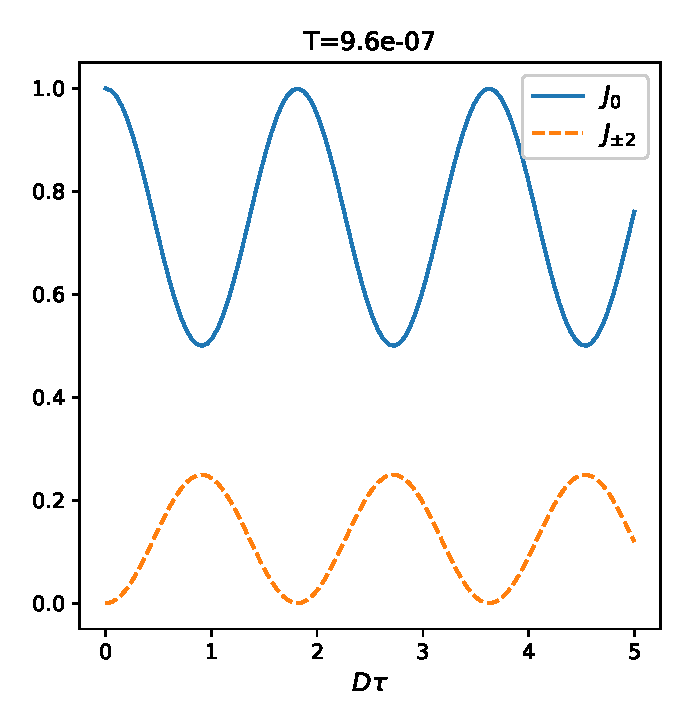
\includegraphics[width=0.5\linewidth]{coherences_n3_beta5.eps}
	\caption{
	  Интенсивности МК~когерентностей~ЯМР~$J_{n}$ ($n=0, 2$) в нанопоре с $N=3$.
      Здесь предполагается, что $\omega_{0} = 2\pi \cdot 500 \cdot 10^{6}$~s$^{-1}$ и $D = 2\pi \cdot 10^{4}$~s$^{-1}$.
	}
	\label{fig:1}
\end{figure}

В этом разделе будет получено точное решение МК~динамики~ЯМР~трехспиновой системы в дипольном упорядоченном состоянии в нанопоре.
Решение будет получена в общем виде, без использования высокотемпературного приближения~\cite{Goldman1970}.
Данная задача аналогична задаче, рассмотренной в разделе~\ref{sec:nanopora-thermodynamic-equilibrium}
для начального термодинамического равновесия в сильном внешнем магнитном поле.

Гамильтониан $H_{MQ}$ уравнения~(\ref{eq:hmq}) состоит из двух блоков для двух возможных значений углового момента спина $(I^2 = S(S+1), \quad S=3/2,1/2)$.
Эти блоки и соответствующие им собственные значения и собственные состояния приведены
в разделе~\ref{sec:sec:nanopora-thermodynamic-equilibrium-exact_sol}.
Матрица плотности системы также состоит из двух блоков $\rho^{3/2}(\tau)$, $\rho^{1/2}(\tau)$, и
%
\begin{equation}
  \label{eq:15}
  \rho^{3/2}(0) = \dfrac 1 Z
  \begin{pmatrix}
    e^{\frac{3b}{2}} & 0 & 0 & 0
    \\
    0 & e^{\frac{-3b}{2}} & 0 & 0
    \\
    0 & 0 & e^{\frac{-3b}{2}} & 0
    \\
    0 & 0 & 0 & e^{\frac{3b}{2}}
  \end{pmatrix},
  \quad
  \rho^{1/2}(0) = \dfrac 1 Z
  \begin{pmatrix}
    	1 & 0
    \\
    0 & 1
  \end{pmatrix}
\end{equation}
%
где $b = \dfrac{\hslash D}{k\mathrm{T}}$ и $T$ --- температура.
Простыми вычислениями можно получить матрицы плотности $\rho^{3/2}(\tau)$ и $\rho^{1/2}(\tau)$,
которые позволяют получить выражение для интенсивности МК~когерентностей~ЯМР.

В рассматриваемых системах появляются только МК~когерентности~ЯМР нулевого и плюс/минус второго порядков.
Интенсивности этих когерентностей равны
%
\begin{equation}
  \begin{split}
    \label{eq:16}
    J_0(\tau) & = 1
    - \dfrac 1 2 \tanh^2\left( \dfrac{3b}{2} \right)
      \sin^2 \left( \sqrt{3} Dt \right),
    \\
    J_{\pm2}(\tau) & = \dfrac{1}{4}
      \tanh^2 \left( \dfrac{3b}{2} \right)
      \sin^2 \left( \sqrt{3} Dt \right)
  \end{split}
\end{equation}
%
Сумма интенсивностей МК когерентностей согласно~(\ref{eq:16}) равна единице в соответствии с уравнением~(\ref{eq:14}).
Зависимости рассчитанных интенсивностей $J_{n}(\tau)$ $(n=0,2)$ от времени эволюции показаны на рисунке~(\ref{fig:1}).

% \subsection{Численный анализ многоспиновой запутанности при различных температурах и различном числе спинов в системе}
\subsection{Температурная зависимость многочастичной запутанности}
\label{sec:5}

В этом разделе приведены результаты полуаналитической симуляции МК эксперимента ЯМР
для модели спин-несущих молекул (атомов) в нанопоре в дипольном упорядоченном состоянии.
Будет рассмотрена зависимость нижней границы квантовой информации Фишера от времени и температуры.
А также получены оценки количества запутанных частиц в системе.
В расчетах предполагается, что $\omega_{0} = 2\pi \cdot 500 \cdot 10^{6}$~s$^{-1}$ и $D = 2\pi \cdot 10^{4}$~s$^{-1}$.

\begin{figure}[H]
 	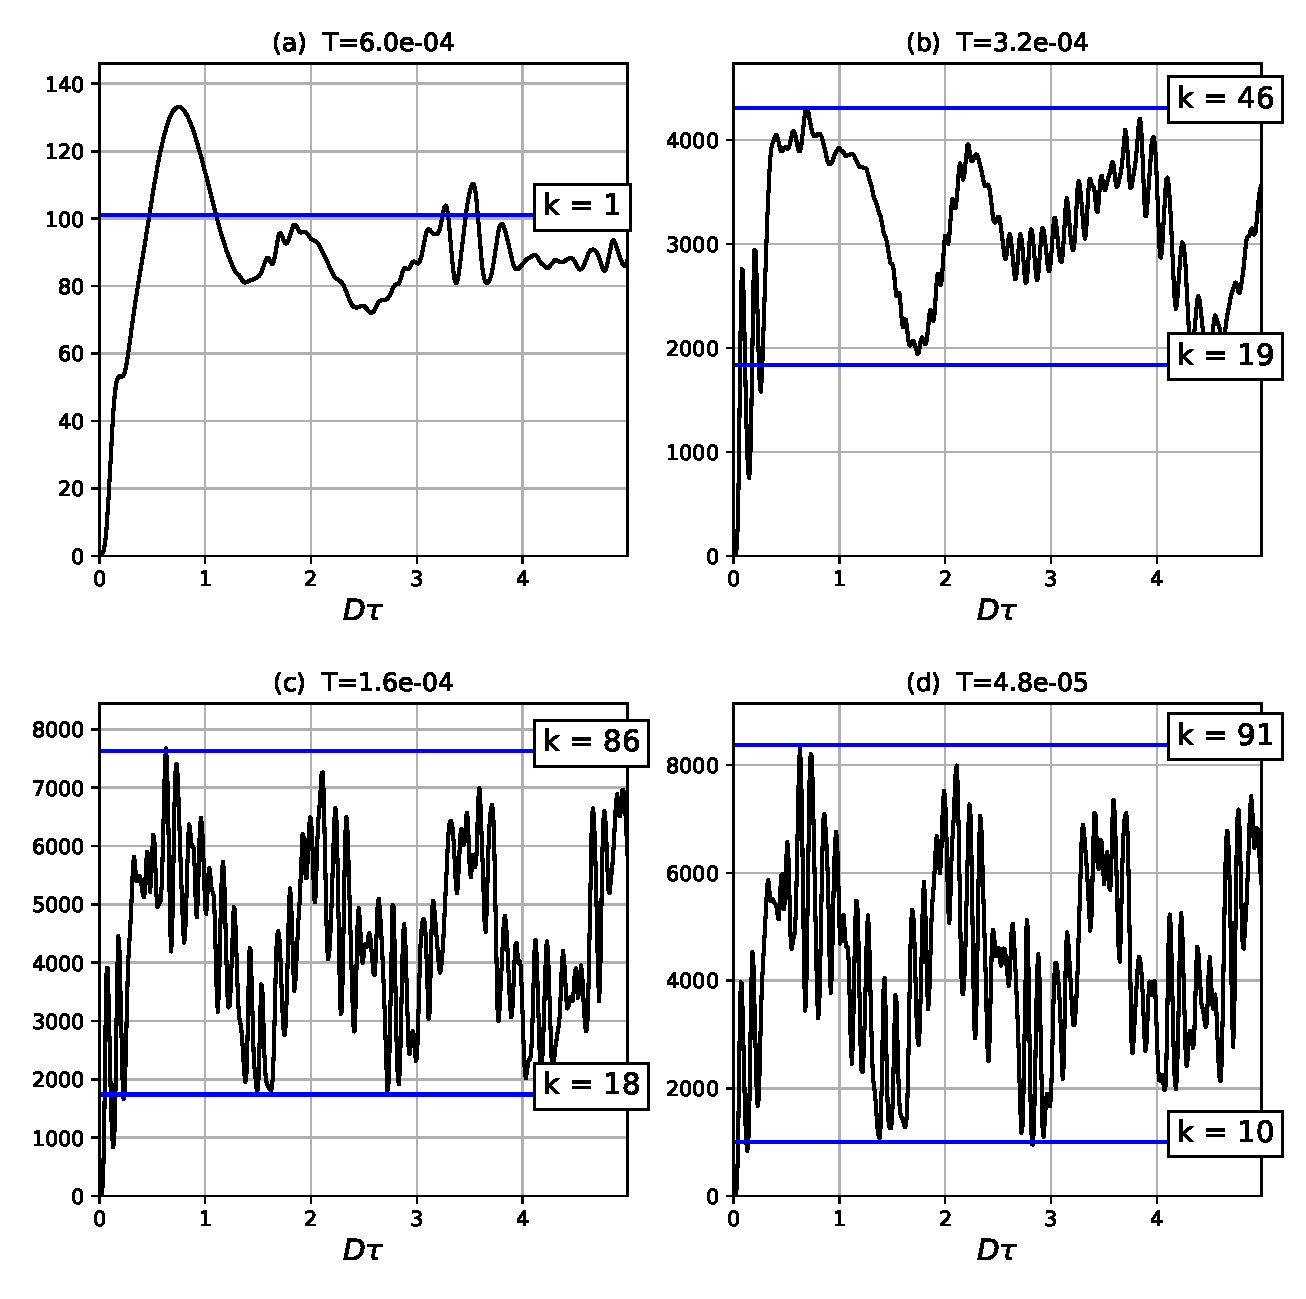
\includegraphics[width=0.95\linewidth]{fisher_low_bound_n101.eps}
	\caption{
	  Зависимость нижней границы  квантовой информации Фишера $F_\mathrm{Q} = 2 M_{2}$
	  от безразмерного времени $D\tau$ при $N=101$.
	  a) $T=6\cdot10^{-4}$~K, неравенство~(\ref{eq:20}) определяет область парной запутанности  (k+1=2), эта область выше горизонтальной линии;
	  b) $T=3.2\cdot10^{-4}$~K, область многоспиновой запутанности представляет собой полосу, ограниченную горизонтальными линиями с~$k=19$~и~$k=46$;
	  c) $T = 1.6\cdot10^{_4}$~K, горизонтальные линии ($k=18$ и $k=86$) ограничивают полосу с многоспиновой запутанностью;
	  d) при $T=4.8\cdot10^{-5}$~K возникают запутанные кластеры с $11-92$ спинами.
	}
	\label{fig:2}
\end{figure}


Рассматриваемая модель спин-несущих молекул (атомов) в нанопоре в дипольном упорядоченном состоянии
расширяет возможности исследования многоспиновой запутанности по сравнению с родственной моделью~(см. раздел~\ref{sec:nanopora-thermodynamic-equilibrium}),
в которой система изначально находилась в термодинамическом равновесии в сильном внешнем магнитном поле.
Модель из раздела~\ref{sec:nanopora-thermodynamic-equilibrium}) неприменима для исследования эволюции системы во времени,
потому что распределение МК~когерентностей~ЯМР~быстро становится стационарным~\cite{Doronin2009}.
Также многоспиновая запутанность изменяется с температурой в очень узком температурном интервале.
Например, все спины запутаны в системе, состоящей из 201 спина уже при температуре $T=6.856\cdot10^{-3}$~K~\cite{Doronin2019}.

Зависимость нижней границы квантовой информации Фишера от времени в системе, состоящей из 101 спина, представлена на Рис.~(\ref{fig:2}) при различных температурах.
Из Рис.~(\ref{fig:2}a) видно, что при температуре $T=6\cdot10^{-4}$~K существует только парная запутанность.
При температуре $T=3.2\cdot10^{-4}$ на Рис.~(\ref{fig:2}b) появляется полоса, в которой неравенство~(\ref{eq:entanglement-criteria}) может быть выполнено, когда $19 \leq k \leq 46$.
Таким образом, существует многоспиновая запутанность в спиновых кластерах, состоящих из 20-47 спинов, при температуре $3.2\cdot10^{-4}$~K.
Когда температура понижается, ширина полосы, в которой существует многоспиновая запутанность, увеличивается.
При температуре $T=1.6\cdot10^{-4}$~K (Рис.~(\ref{fig:2}c)) появляются кластеры из 19-87 запутанных спинов, а при температуре $T=4.8\cdot10^{-5}$~K (Рис.~(\ref{fig:2}d)), наблюдаются 11-92 запутанных спина.

\begin{figure}
 	\includegraphics[width=0.95\linewidth]{entangled_spins_by_n.eps}
	\caption{
	  Зависимость максимального количества запутанных спинов,
	  усредненного по времени эволюции $(0 \leq D\tau \leq 3)$,
	  от температуры при  a) $N=51$; b) $N=75$; c) $N=101$.
	}
	\label{fig:3}
\end{figure}

Зависимость максимального числа запутанных спинов за время эволюции $({0}\leq \mathrm{D}\tau\leq{3})$ от температуры при разных числах спинов в нанопоре представлена на Рис.~(\ref{fig:3}).
Максимальное количество запутанных спинов уменьшается при повышении температуры.
Максимальное количество запутанных спинов увеличивается, когда увеличивается число спинов в нанопоре, потому что система в нанопоре становится плотнее.

\section{Выводы}
\label{sec:conslusions}
% We investigated many-particle entanglement in MQ NMR spectroscopy using a nanocavity filled with spin-carrying atoms (molecules).
% We developed a theory of MQ NMR in a nanocavity at low temperatures.
% The theory is based on the idea that  molecular diffusion is substantially faster than the time of the spin flip-flop processes.
% As a result, the problem is reduced to a system of equivalent spins [23, 25], which can be analyzed in the basis of the common eigenstates of the total spin angular momentum and its projection on the external magnetic field.
% Since there is a connection between the second moment (dispersion) of the distribution of the MQ NMR intensities and many-spin entanglement [17], we extracted information about many-spin entanglement from the MQ NMR spectrum. The temperature dependence of many-spin entanglement was also investigated.
% \par
% The main lesson consists in significant growth of many-particle entanglement at low temperatures.
% All or almost all spins are entangled at the dimensionless temperature $\frac{1}{b}$ of the order of 1.
% This suggests that $k$-entangled states with large $k$ emerge in a typical MQ NMR system at low temperatures.
% This is particularly interesting given the absence of entanglement in the initial state. We expect such behavior to be typical for MQ NMR.
% \par
% We can conclude that MQ NMR spectroscopy is an effective method for the investigation of many-spin entanglement and the spreading of MQ correlations inside many-spin systems. It can be used for experimental investigations of quantum information processing in solids (note a related study of decoherence in liquids \cite{HOU2017863}).
% \par

В этой главе была исследована многочастичная запутанность в МК спектроскопии ЯМР в нанопоре, заполненной сотнями спин-несущими частицами.
Для этого была разработана МК теория ЯМР в нанопоре при низких температурах.
Было рассмотрено два начальных состояния системы:
термодинамически равновесное
и дипольное упорядоченное.
В обоих случах впервые удалось исследовать температурную зависимость многочастичной запутанности.
Все или почти все спины запутаны при безразмерной температуре $\frac{1}{b}$ порядка 1.
Это говорит о том, что $k$-запутанные состояния с большим $k$ возникают в типичной системе МК ЯМР при низких температурах.
Это особенно интересно, учитывая отсутствие запутанности в начальном состоянии.
Можно заключить, что такое поведение типично для МК ЯМР.
Так же была исследована зависимость многоспиновой запутанности
от количества спинов в нанопоре.
Показано, что с ростом количества спинов в нанопоре,
скорость возникновения запутанных кластеров при понижении температуры увеличивается.

Результаты этого раздела наглядно демонстрируют
универсальность разработанного в этой диссертации метода исследования многочастичной запутанности.


\section{Многочастичная запутанность в квазиодномерных цепочках}
\begin{frame}{Однородная цепочка спинов}
  \begin{columns}
    \column{0.35\textwidth}
    \begin{figure}
      \includegraphics[width=\textwidth]{sample-fap-crystal-structure-part.png}
      \caption{Фтористый апатит Ca$_{10}$(PO$_4$)$_6$F$_2$}
    \end{figure}

    \column{0.6\textwidth}
      Часть кристаллической структуры FAp, показывающая окружение атомов фтора.
      Атомы кислорода были удалены для ясности.
      Атомы фтора равномерно разнесены ($r_{FF}= 3.44$\AA) и расположены в колонны вдоль $c$-оси кристалла.
      Каждый атом фтора окружен тремя равноудаленными атомами фосфора при $r_{FP} = 3.67$\AA,
      которые расположены в вершинах равносторонних треугольников на плоскости, перпендикулярной к $c$-оси,
      а также тремя ионами Ca\textrm{II} на расстоянии $2.34$\AA.
  \end{columns}
\end{frame}
\note{
  Фтористый апатит.
}

\begin{frame}{Альтернированная цепочка}
\begin{columns}

    \column{0.3\textwidth}
    \begin{figure}
    \includegraphics[width=1.0\textwidth]{model-zigzag-chain-schema.png}
    \caption{}
    \end{figure}

    \column{0.6\textwidth}
    \begin{block}{Константы взаимодействия}
        $$D_1=\dfrac{\gamma^2\hbar }{r^3}, $$
        $$D_2 = D_1\dfrac{ 3\cos^2 \varphi -1 }{2} $$
        $$D_3 = D_1 \dfrac{ 3\sin^2 \frac{\varphi}{2} -1}{16 \sin^3, \frac{\varphi}{2}}$$
        где $\gamma$ - гиромагнитное отношение,
        $\varphi$ - угол между соседними связями,
        $r$ - расстояние между соседними спинами в цепочке.
    \end{block}

\end{columns}
\end{frame}
\note{
    Базовый случай это когда одна линия связи направлена вдоль поля. тогда констаты будет самой большой в доль поля.
    Изменяя угол к полю мы можем получить как альтернированную цепочку так и однородную.
    В приближении ближайших и следующих соседей, задача решается аналитически, но она
    не дает полной картины. Поэтому мы решали данную систему численно.
}

\begin{frame}{Альтернированная цепочка (JMR-20)\footnote[frame]{
        G.A. Bochkin and et al., \textit{J. Magn. Res.} \textbf{319}, 106816, (2020)}}
\begin{columns}

    \column{0.4\textwidth}
    \begin{figure}
      \includegraphics[width=0.85\textwidth]{model-zigzag-chain-hambergite-structure.png}
      \caption{}
    %\caption{Hанопора со спин-несущих молекулами во внешнем сильном магнитном поле $\vec B$}
    \end{figure}

    \column{0.6\textwidth}
    \begin{block}{Гамбергит $Be_2BO_3(OH)$ }
        \begin{itemize}
            \item Дипольное взаимодействия между ближайшими спинами протонов в цепи в 17 раз сильнее, чем со спинами окружающих цепей (в худшем случае).
            \item Взаимодействия с остальными окружающими спинами по меньшей мере в 30 раз слабее.
            \item Вклад дипольной связи между спинами в одной и той же цепи доминирует над остальными взаимодействиями.
        \end{itemize}
    \end{block}

\end{columns}
\end{frame}
\note{
    В одномерных цепочках возникают когерентности только $\pm 2$ порядка
    и следовательно дисперсия распределения будет небольшой
    и мы не увидим запутанных кластеров.
    Однако в альтернированная цепочке гамбергита возникают когерентности $\pm 4$ порядка
    и следовательно можно использовать эту модель для исследования многочастичной запутанности.
    The distance to these two protons is 4.49 Å
    The distance between a given chain and surrounding proton chains is at least 2.1 times larger than the distance between neighbors in the chain.

  % JMR 2020
}
\begin{frame}{Эволюция нижней границы информации Фишера}
% (AMR-20)\footnote{G.A. Bochkin et al., \textit{Appl. Magn. Res.} \textbf{51}, 667-678, (2020)}
\begin{columns}

    \column{0.6\textwidth}
    \begin{figure}
    \includegraphics[width=0.95\textwidth]{result-zchain-m2-by-time-n6-beta10.eps}
    %\caption{Hанопора со спин-несущих молекулами во внешнем сильном магнитном поле $\vec B$}
    \end{figure}

    \column{0.4\textwidth}
    Зависимость нижней границы квантовой информации Фишера
    $$ F_Q = 2M_2(\tau, T) $$
    от безразмерного времени $D_1 \tau$
    для шести спинов
    при температуре $T = 2.5 \times 10^{-3}$ $(\beta = 10)$.
    Область многочастичной запутанности ограничена горизонтальными линиями $k = 1$, $k = 5$.
\end{columns}
\end{frame}
\note{
   Мы не можем точно сказать сколько спинов запутанно,
   но можем дать нижнюю оценку на количество запутанных между собой спинов.
}


\begin{frame}{Максимальное количество запутанных спинов}
\begin{columns}

    \column{0.5\textwidth}
    \begin{figure}
    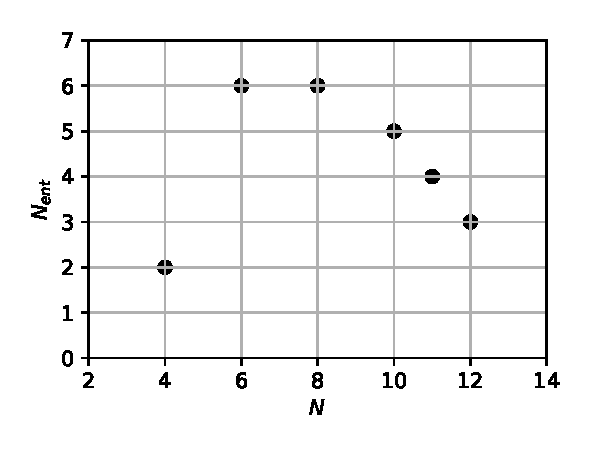
\includegraphics[width=\textwidth]{result-zchain-nent-by-n-beta10.eps}
    \caption{}
    \end{figure}

    \column{0.5\textwidth}
    Зависимость максимального количества запутанных спинов $N_\mathrm{ent}$ от длины цепи при температуре $T = 2.5 \times 10^{-3}$ $(\beta = 10)$.

    \vspace{0.5cm}

    \alert{Создание запутанных кластеров в рассматриваемых зигзагообразных цепочках ограничено слабыми дипольными взаимодействиями удаленных спинов}.
\end{columns}
\end{frame}
\note{
  Установлено что, при фиксированной температуре с ростом числа спинов в цепи размер запутанных кластеров может уменьшаться;
}


\begin{frame}{Максимальное количество запутанных спинов}
  \begin{columns}
     \column{0.5\textwidth}
     \begin{figure}
     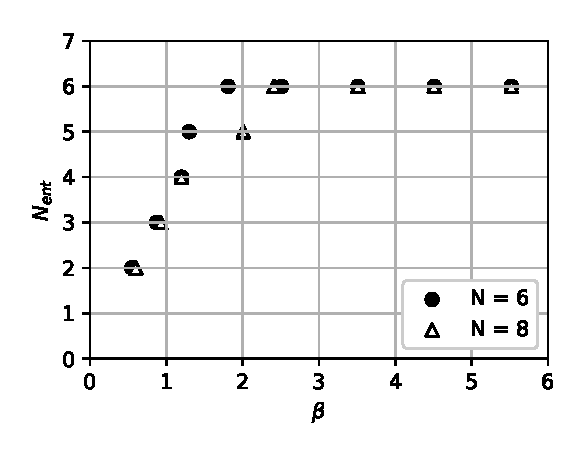
\includegraphics[width=\textwidth]{result-zchain-nent-by-beta-n8-n6.eps}
     \caption{}
     \end{figure}

     \column{0.45\textwidth}
     \begin{block}{}
       Зависимость максимального количества запутанных спинов $N_\mathrm{ent}$ от обратной температуры
       $$ \beta = \dfrac{\hbar\omega_0}{kT} $$
       в зигзагообразной цепочки из 6 и 8 спинов.
    \end{block}
  \end{columns}
\end{frame}
\note{
    Для 6 спинов накачка происходит быстрее, чем для 8 спинов.
}


\section{Измерение информации Вигнера-Янасе в МК эксперименте ЯМР}
\chapter{Измерение информации Вигнера-Янасе в МК эксперименте ЯМР}
\label{chapter:wyi-mesuarement}

% PLA-2021

% \section{Многоквантовая динамика при низких температурах}
% \input{results/mq-dynamic-at-low-temperature}
%
% \section{Многоспиновая запутанность в системе эквивалентных спинов}
% \input{models/equivalent-spins}
% \input{results/equivalent-spins-entanglement-with-term-equilibrium-state}
% \input{results/equivalent-spins-entanglement-with-dipolar-ordered-state}
%
% \section{Многоспиновая запутанность в цепочках}
% \input{models/zigzag-spin-chain}
% \input{results/zigzag-spin-chain-entanglement}
%
% \section{Определение информации Вигнера-Янасе в МК эксперименте ЯМР}
% \input{results/determination-of-wigner-yanase-information}
%
% \section{Сравнение информации Вигнера-Янасе и Фишера}
% \input{results/comparison-wyi-and-fi}

\section{Итоги}
\item
Разработана теория МК ЯМР в системе эквивалентных спинов s=1/2 при произвольных температурах. При низких температурах эта теория применена для расчетов многоспиновой запутанности в
нанопоре и зигзагообразной цепочке. 
Проведенные исследования позволяют заключить, что МК-спектроскопия ЯМР является тонким и полезным методом для исследования различных проблем квантовой информатики.

\item
Исследована температурная зависимость многочастичной запутанности в нанопоре с термодинамическим равновесным зеемановским и дипольно упорядоченным начальными состояниями. 
С понижением температуры количество запутанных спинов растет.
При температуре
$T = 6.856\cdot10^{-3}$~K $(\beta=3.5)$
почти все спины (до 179 из 201) запутаны. 
Можно заключить, что в типичной системе МК ЯМР при низких температурах возникают многочастичные запутанные состояния,
даже при отсутствии запутанности в начальном состоянии.  


\item
Исследована многочастичная запутанность в квазиодномерных цепочках ядерных спинов в зависимости от параметров цепи и температуры.
В однородных цепочках детектируется только парная запутанность, что согласуется с результатами, представленными в литературе.
В зигзагообразной цепочке при низких температурах почти все спины запутанны, так же как и в нанопоре.

\item
Предложен метод экспериментального измерения точного значения косой информации Вигнера-Янасе в рамках МК спектроскопии ЯМР.
Разработанный метод позволяет не только исследовать многочастичную запутанность методами МК ЯМР,
но и открывает возможность решения широкого класса задач квантовой теории информации.

% \input{suplemental-materials}

\end{document}